\subsection{Schutzmechanismen}

Im Kapitel Schutzmechanismen befassen wir uns mit dem Thema, wie man unsere anfällige trainierten Modelle aus Kapitel \ref{chap:modelltraining} fine tunen bzw. Schutzmechanismen anwenden, um das Modell robuster gegenüber unsere adversarial Training machen:

\subsubsection{Data Augmentation}

Bei der Data Augmentation verändern wir mit einer zufälligen Transformation die vorhandenen Trainingsdaten, um die Variabilität im Datensatz zu erhöhen. Dies kann durch verschiedene Methoden geschehen, wie zum Beispiel:

\begin{itemize}
    \item \textbf{Rotation}: Drehen des Bildes um einen bestimmten Winkel.
    \item \textbf{Verschiebung}: Verschieben des Bildes in eine bestimmte Richtung.
    \item \textbf{Skalierung}: Ändern der Grösse des Bildes.
    \item \textbf{Spiegelung}: Spiegeln des Bildes entlang einer Achse.
    \item \textbf{Rauschen hinzufügen}: Zufälliges Rauschen hinzufügen, um das Bild zu verändern.
\end{itemize}

Diese Techniken helfen, das Modell robuster zu machen und die Generalisierungsfähigkeit zu verbessern, indem sie es zwingen, verschiedene Variationen der Daten zu lernen.

\subsubsection{Input Ensembles}

Mit Input Ensembles nutzen wir mehrere Modelle, die unabhängig voneinander trainiert wurden. Der Prozess sieht wie folgt aus:

\begin{enumerate}
    \item \textbf{Training mehrerer Modelle}: Jedes Modell wird separat mit demselben Trainingsdatensatz trainiert.
    \item \textbf{Unabhängige Vorhersagen}: Jedes Modell gibt eine eigene Vorhersage, basierend auf dem Input.
    \item \textbf{Kombinieren der Vorhersagen}: Der endgültige Output wird durch Mehrheitsentscheidung (Voting) bestimmt. 
\end{enumerate}

Durch diese Methode können wir die Genauigkeit und Robustheit der Vorhersagen verbessern.

\subsubsection{Adversarial Training} \label{chap:adversarial training}

Beim Adversarial Training nutzen wir unsere generierten \acrlong{uap} und fügen diese im Preprocessing-Schritt mit einer Wahrscheinlichkeit von 50 \% zu den Eingabedaten hinzu. Der Ablauf ist wie folgt:

\begin{enumerate}
    \item \textbf{Generierung der UAPs}: Erstellen von adversarial Beispielen, die speziell darauf ausgelegt sind, das Modell zu täuschen, gemäss Kapitel \ref{chap:UAP}.
    \item \textbf{Integration in das Training}: Diese adversarial Beispiele werden während des Trainingsprozesses in die Eingabedaten integriert.
    \item \textbf{Training mit robusteren Daten}: Das Modell lernt, auch in Anwesenheit dieser adversarial Beispiele korrekte Vorhersagen zu treffen.
\end{enumerate}


\subsubsection{Übersicht Modell Finetuning}
In der Abbildung \ref{fig:Evaluierungspipeline} ist der Iterationsschritt der Pipeline zu sehen. Die Pipeline wird dabei x-mal durchlaufen, was bedeutet, dass die Robustifizierung ebenfalls x-mal für das Modell und Datensatz durchgeführt wird.

\begin{figure}[H]
    \centering
    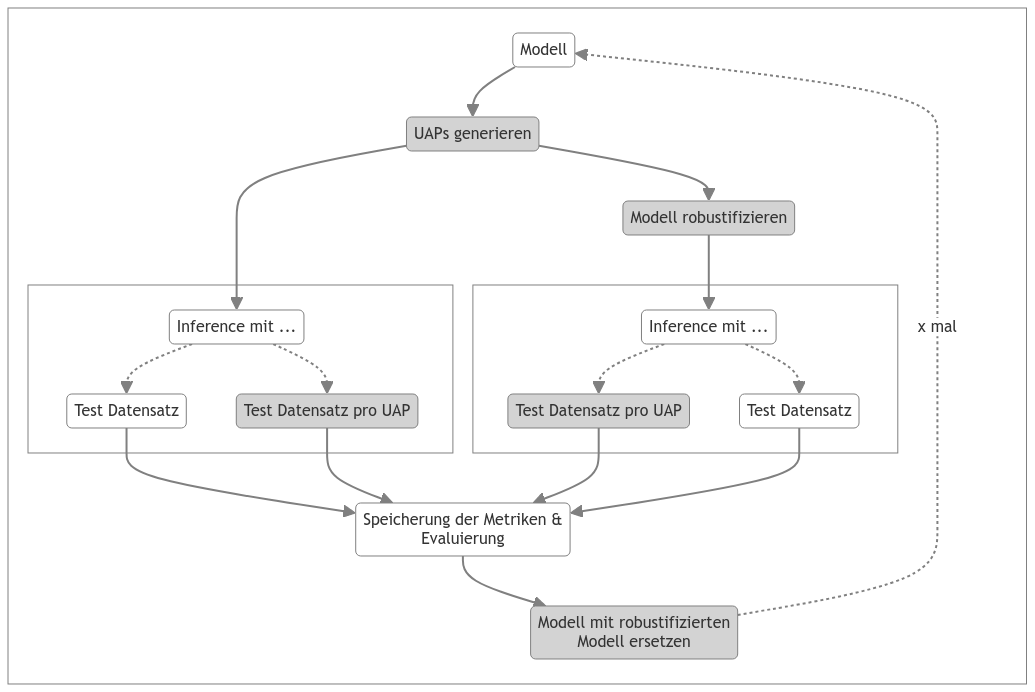
\includegraphics[width=\linewidth]{01-images/04-methodik/robustifizierungs-pipeline.png}
    \caption{Übersicht der Evaluierungspipeline}
    \label{fig:Evaluierungspipeline}
\end{figure}

\begin{itemize}
    \item \textbf{Modell}: Startpunkt der Pipeline, unser trainiertes Modell auf unserem Datensatz.
    \item \textbf{UAPs generieren}: \acrshort{uap} werden generiert, um das Modell robuster zu machen.
    \item \textbf{Modell robustifizieren}: Adversarial Training wird angewendet, um das Modell zu robustifizieren. Siehe Kapitel \ref{chap:adversarial training}.
    \item \textbf{Inference mit...}: Erfolgt über zwei parallele Wege:
        \begin{itemize}
            \item Einer führt zur Inferenz mit dem ursprünglichen Modell, jeweils für den Testdatensatz mit und ohne \acrshort{uap}.
            \item Der andere Weg führt zur Inferenz mit dem robustifizierten Modell, ebenfalls für Testdatensatz mit und ohne \acrshort{uap}.
        \end{itemize}
    \item \textbf{Speicherung der Metriken \& Evaluierung}: Hier speichern wir die berechneten Metriken und vergleichen die vier Outputs der Inferenz miteinander untereinander für jede Robustifikations Iteration. 
\end{itemize}

\newpage

\subsubsection{Pseudocode für die Pipeline}

\begin{algorithm}
\caption{Pipeline zur Generierung universeller adversativer Störungen (UAP)}
\label{alg:UAP_Pseudo_Algorithmmus}
\begin{algorithmic}[1]
\REQUIRE modelname, dataset, n\_robustifications, i, n, t, p, lambda\_norm, r, eps, lr\_uap, seed, num\_workers, device, verbose
\STATE Initialisiere Modell und Hyperparameter
\FOR{\texttt{jede Robustifizierung k in n\_robustifications}}
    \STATE Definiere Modellordner
    \STATE Überprüfe und lade vorhandene robustifizierte Modelle, falls verfügbar
    \IF{Robustifizierung muss generiert werden}
        \STATE Logge die Generierung von UAP
        \STATE Generiere UAPs und logge sie
        \STATE Bewerte das Modell auf Testdaten ohne UAP
        \FOR{\texttt{jeden Störungsindex bis zu i}}
            \STATE Bewerte das Modell auf Testdaten mit UAP
        \ENDFOR
        \STATE Entfriere und trainiere das Modell zur Robustifizierung
        \STATE Speichere und lade den besten Modell-Checkpoint
        \STATE Bewerte das robustifizierte Modell auf Testdaten
        \FOR{\texttt{jeden Störungsindex bis zu i}}
            \STATE Bewerte das robustifizierte Modell auf Testdaten mit UAP
        \ENDFOR
    \ENDIF
\ENDFOR
\end{algorithmic}
\end{algorithm}
